% Requires IEEEtran, graphicx and amsmath. Copy this file with figures/ and the two table .tex files.

\section{Numerical Results and Discussion}\label{sec:numerical_mobility}

The numerical results in this section are preliminary effective-Gaussian diagnostics: fading enters through $T_{\rm eff}=\langle\sqrt{\eta}\rangle^2$, while fading-induced variance is omitted. They are not a certified fading-channel security lower bound or a finite-size-secure key yield.

We use a $10\times10$ grid of 100 cell centers in a $1\,\mathrm{km}\times1\,\mathrm{km}$ UAV region, 30 slots of 20 s, and $v_{\max}=15$ m/s. The HAP/UAV altitudes are 20/1 km. The demonstrative HAP embedding preserves the 21.9393102292-km reference link. A synthetic cloud at 5 km has radius 420 m, attenuation 10 dB, initial center $(2093.71686623,450)$ m and velocity $(3,0)$ m/s. These cloud parameters are not measured weather data.

At each position/state, source selection enumerates 197 authenticated MB sources without interpolating $C,w$ or SKR. The same ideal heterodyne receiver, $\xi_{\rm ch}=0.0186$, $\beta_{\rm rec}=0.95$, source adaptation and cloud scenario are used in all schemes. The UAV trajectory is optimized by DP on the finite grid. The implemented objective is $\overline S-\lambda D_{\rm fly}/D_{\rm ref}$ with $D_{\rm ref}=1000$ m; it is a distance penalty, not a propulsion-energy model.

\begin{table}[t]
\caption{System and synthetic demonstration parameters. HAP coordinates preserve the reference link; cloud parameters are not measured weather data.}
\label{tab:mobility_system}
\centering\scriptsize
\begin{tabular}{ll}\hline
Parameter & Value \\ \hline
HAP altitude & 20000\,m \\
UAV altitude & 1000\,m \\
UAV region & 1000 x 1000\,m\textasciicircum{}2 \\
Candidate positions & 100 \\
Grid spacing & 100\,m \\
Reference slant distance & 21.93931\,km \\
Time slots & 30 \\
Mission duration & 600\,s \\
Slot duration & 20\,s \\
Maximum UAV speed & 15\,m/s \\
Cloud altitude & 5000\,m \\
Cloud radius & 420\,m \\
Cloud attenuation & 10\,dB \\
Cloud initial center & [2093.7168662297536, 450.0]\,m \\
Cloud velocity & [3.0, 0.0]\,m/s \\
MB source candidates & 197 \\
Uniform source candidates & 30 \\
Reconciliation efficiency & 0.95 \\
Optical wavelength & 1550\,nm \\
Full divergence & 10\,microrad \\
Beam waist & 0.098676065\,m \\
Receiver diameter & 0.55\,m \\
Clear zenith transmission & 0.92 \\
HAP angular jitter & 15.61\,microrad \\
Input channel excess noise & 0.0186\,SNU \\
Detector efficiency & 1 \\
Detector excess noise & 0\,SNU \\
Ideal heterodyne chi & 1 \\
Movement reference distance & 1000\,m \\
Main movement penalty & 0.001\,bits/use \\
\hline\end{tabular}
\end{table}


\begin{table*}[t]
\caption{Preliminary effective-Gaussian performance. Availability means the fraction of slots with $S_n>0$; it is not an operational QKD no-outage probability. Own objectives use the scheme's displayed penalty; the common-penalty row permits like-for-like comparison.}
\label{tab:mobility_performance}
\centering\footnotesize
\begin{tabular}{lrrrr}\hline
Metric & S1 & S2 & S3 & S4 \\ \hline
Average SKR (bits/use) & 0.033503392 & 0.053493459 & 0.061883254 & 0.061041914 \\
Improvement vs S1 (\%) & 0 & 59.665802 & 84.70743 & 82.196221 \\
Improvement vs S2 (\%) & -37.369181 & 0 & 15.683777 & 14.110986 \\
Positive-rate slots (\%) & 100 & 100 & 100 & 100 \\
Flight distance (m) & 0 & 0 & 2323.6068 & 600 \\
Movement penalty (bits/use) & 0 & 0 & 0 & 0.001 \\
Own penalized objective (bits/use) & 0.033503392 & 0.053493459 & 0.061883254 & 0.060441914 \\
Objective at common lambda=0.001 & 0.033503392 & 0.053493459 & 0.059559647 & 0.060441914 \\
\hline\end{tabular}
\end{table*}


\subsection{Positioning and mobility}

The reference fixed UAV gives 0.0335034 bits/use. The optimized stationary UAV selects $(950,950)$ m and gives 0.0534935 bits/use, a 59.67\% improvement. Without clouds, the cached clear-state optimum is $(950,450)$ m: the boundary solution therefore reflects geometry and cloud exposure, not an assumed grid error. No optimum outside the finite region is claimed.

The maximum-SKR moving trajectory gives 0.0618833 bits/use and a flight distance of 2323.61 m. With $\lambda=0.001$ bits/use, S4 gives 0.0610419 bits/use while flying 600 m. It retains 98.64\% of S3's average SKR with 74.18\% less flight distance; its gains over S1 and S2 are 82.20\% and 14.11\%, respectively. Its own penalized objective is 0.0604419 bits/use and is not directly equated with an unpenalized mean.

Figs.~\ref{fig:mobility_ieee_1} and \ref{fig:mobility_ieee_2} show how cell changes avoid most cloud attenuation. Per-slot discontinuities are retained. Fig.~\ref{fig:mobility_ieee_3} uses the normalized sum $C(n)=N_t^{-1}\sum_{k=1}^n S(k)$, whose endpoint is the average SKR; an unvalidated channel-use rate is not assumed.

\subsection{SKR--mobility trade-off and source adaptation}

Fig.~\ref{fig:mobility_ieee_4} shows only the eight evaluated penalty solutions, with overlapping points identified by their CSV penalty values. It is not an interpolated continuous Pareto frontier. Fig.~\ref{fig:mobility_ieee_5} varies only speed along $+x$ in the original cloud scenario; no monotonic trend is assumed. Additional fixed starting-position/direction sensitivities are reported separately as descriptive scenario means and standard deviations, not confidence intervals.

Fig.~\ref{fig:mobility_ieee_6} compares the exact selected $(\nu_{\rm MB,raw},V_A)$ of S2 and S4. The repository uses $\nu_{\rm repo}=42.5\nu_{\rm raw}$. Changes occur at selected cloud/mobility states, and repeated parameter values are retained rather than interpolated.

\subsection{Uniform versus MB and limitations}

For the stationary case, optimized Uniform gives 0.0045255 bits/use and optimized MB gives 0.0534935 bits/use (absolute gain 0.0489679 bits/use).

For the moving lambda0 case, optimized Uniform gives 0.0052217 bits/use and optimized MB gives 0.0618833 bits/use (absolute gain 0.0566615 bits/use).

Uniform enumerates 30 valid source variances and MB enumerates 197 shaping/variance pairs under common channel and mobility conditions. This supports a joint source-adaptation comparison; it does not isolate shaping at matched modulation energy or certify a continuous source optimum.

The omitted output term is $(\langle\eta\rangle-T_{\rm eff})V_A$. In addition, replacing $\langle\eta\rangle\xi_{\rm ch}$ by $T_{\rm eff}\xi_{\rm ch}$ removes $(\langle\eta\rangle-T_{\rm eff})\xi_{\rm ch}$. Thus the full moment-matched Bob variance exceeds the adopted variance by $(\langle\eta\rangle-T_{\rm eff})(V_A+\xi_{\rm ch})$. Full-fading mixture precision and operational security justification remain unresolved, so these Gaussian diagnostics cannot support final fading-security conclusions.

The circular binary-cloud model, known cloud schedule/CSI, instantaneous source adaptation, and endpoint slot-rate approximation neglect cloud fluid dynamics, estimation errors, propagation during transitions and reacquisition overhead. Positive-rate-slot availability is not physical no-outage probability. All reported optima are restricted to the discrete grid and available numerical source catalogs.

\begin{figure*}[t]

\centering

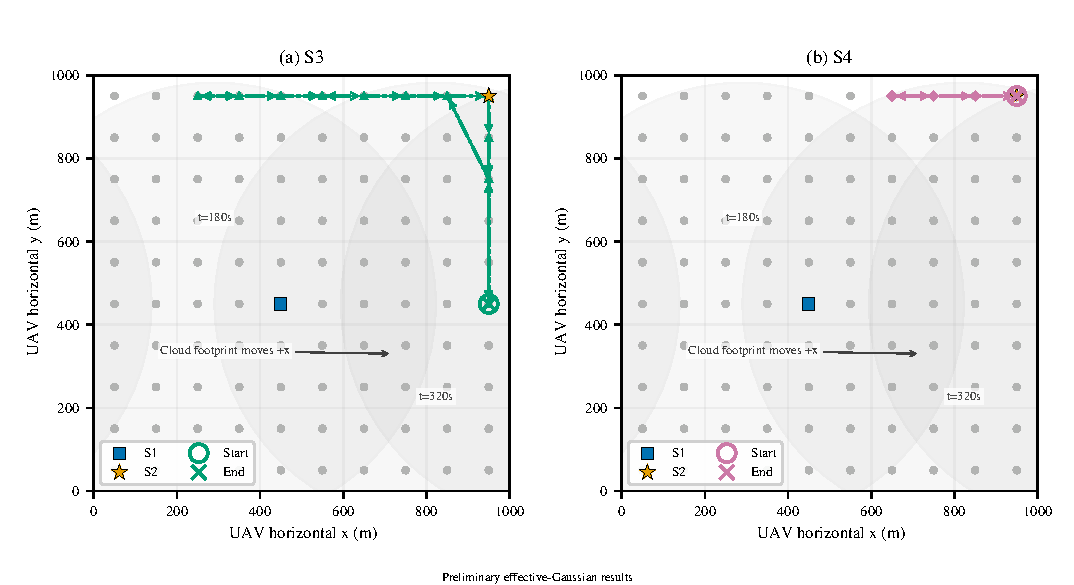
\includegraphics[width=\textwidth]{figures/figure_1_cloud_trajectories_double.pdf}

\caption{Cloud-induced occlusion and trajectories: (a) S3, (b) S4. Gray circles are occlusion footprints mapped through the altitude-plane ray intersection into UAV coordinates, not clouds located at UAV altitude. For a=(h\_c-h\_U)/(h\_H-h\_U), their centers are (c-a q\_H)/(1-a) and radii R\_c/(1-a). Actual cloud centers at h\_c=5 km and UAVs at h\_U=1 km are stored in the plotting CSV. Arrows indicate movement; open circles and crosses show start/end, which may coincide.}\label{fig:mobility_ieee_1}

\end{figure*}

\begin{figure}[t]

\centering

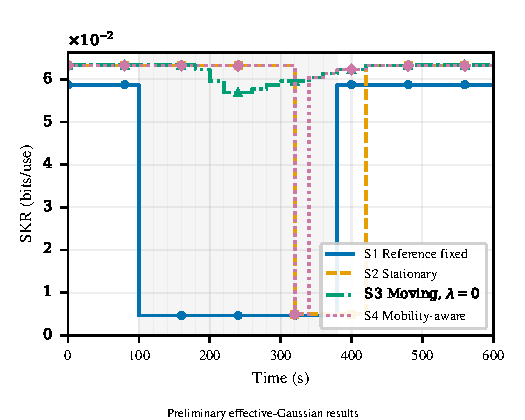
\includegraphics[width=\columnwidth]{figures/figure_2_skr_time_single.pdf}

\caption{Original per-slot usable SKR for S1--S4, with post-step rendering and no smoothing. Gray intervals indicate cloud blockage of the reference optical path. All results use the same preliminary effective-Gaussian channel, source adaptation, beta=0.95 and ideal heterodyne receiver.}\label{fig:mobility_ieee_2}

\end{figure}

\begin{figure}[t]

\centering

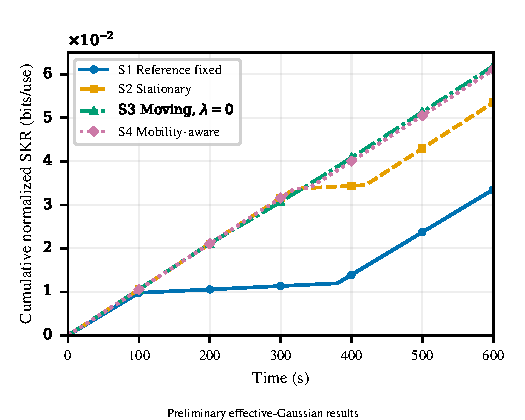
\includegraphics[width=\columnwidth]{figures/figure_3_cumulative_normalized_single.pdf}

\caption{Cumulative normalized SKR C(n)=sum\_{k=1}\textasciicircum{}n S(k)/N\_t, with C(0)=0 and C(N\_t) equal to the mean usable SKR. No channel-use rate is specified, so these values are in bits/use, not total secret bits or finite-size-secure key yield.}\label{fig:mobility_ieee_3}

\end{figure}

\begin{figure}[t]

\centering

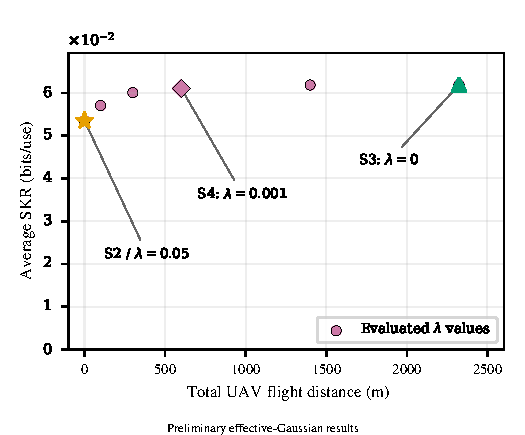
\includegraphics[width=\columnwidth]{figures/figure_4_skr_flight_tradeoff_single.pdf}

\caption{Average SKR versus total flight distance for all eight evaluated movement penalties. Only evaluated points are drawn; overlapping lambda values remain separately listed in CSV. S2, S3(lambda=0) and S4(lambda=0.001 bits/use) are marked. Flight distance is not propulsion energy; average SKR and penalized objective are reported separately.}\label{fig:mobility_ieee_4}

\end{figure}

\begin{figure}[t]

\centering

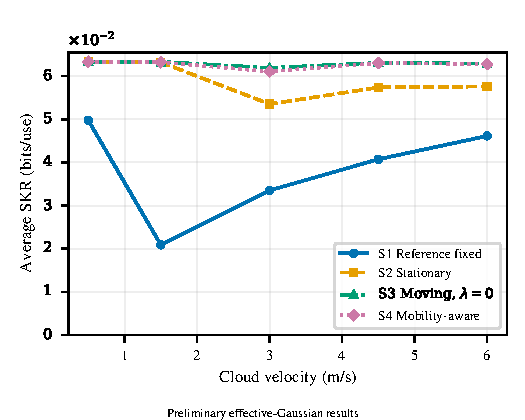
\includegraphics[width=\columnwidth]{figures/figure_5_cloud_velocity_single.pdf}

\caption{The five original cloud-speed cases with fixed +x direction and unchanged initial center, radius, attenuation, physical channel and mission. Curves connect only evaluated speed points for visual guidance, without interpolation or extrapolated results. No monotonicity is asserted.}\label{fig:mobility_ieee_5}

\end{figure}

\begin{figure}[t]

\centering

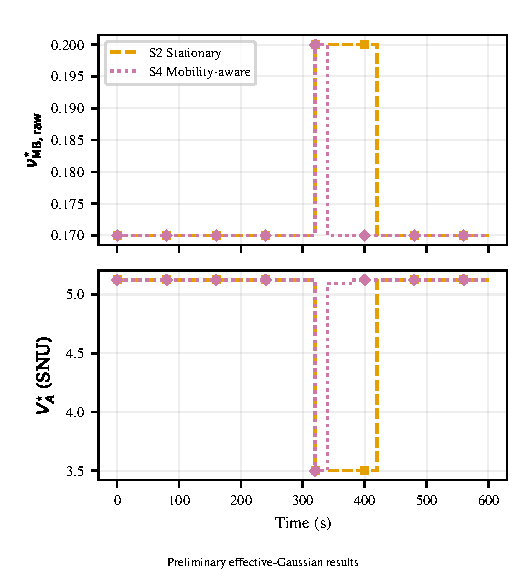
\includegraphics[width=\columnwidth]{figures/figure_6_source_parameters_single.pdf}

\caption{Exact selected source pairs for S2 and S4: (a) nu\_MB,raw and (b) V\_A. Values are held over each slot, without interpolation. The repository convention is nu\_repo=42.5 nu\_raw. Both schemes use identical source-adaptation rules and the same finite MB catalog.}\label{fig:mobility_ieee_6}

\end{figure}

\begin{figure}[t]

\centering

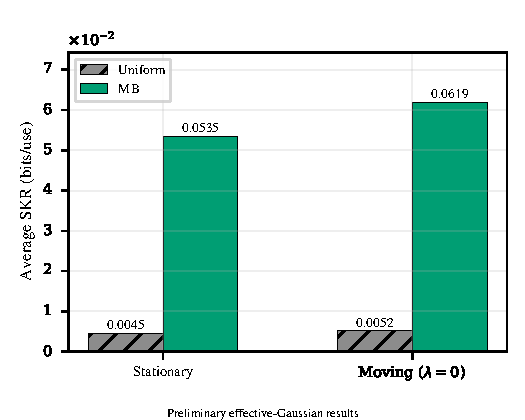
\includegraphics[width=\columnwidth]{figures/figure_7_uniform_mb_single.pdf}

\caption{Controlled optimized Uniform and MB comparison for stationary and moving(lambda=0) UAVs. Uniform optimizes VA over 30 authenticated Uniform sources; MB optimizes nu\_raw and VA over 197 authenticated MB sources. Geometry, clouds, slots, receiver, noise and mobility constraints are common. Available catalog sizes and selected energy may differ; this is a joint source-adaptation comparison, not an isolated energy-matched shaping gain.}\label{fig:mobility_ieee_7}

\end{figure}
